\documentclass{article}

\usepackage{tikz}
\usepackage{standalone}
\usepackage{pgfplots}
\pgfplotsset{compat=newest}
\usepackage{tikz}
\usetikzlibrary{decorations.markings}
\usetikzlibrary{patterns}

\usepackage{subcaption}
\usepackage[margin=2.5cm]{geometry}
\usepackage{amsmath}
\usepackage{amssymb}


\newcommand\greybox[1]{
	\vskip\baselineskip
	\par\noindent\colorbox{lightgray}{
		\begin{minipage}{\textwidth}#1\end{minipage}
	}
	\vskip\baselineskip
}

\title{Forelesning 2}


\begin{document}
\maketitle

\section{Schrödinger ligningen}

Vi starter med å skrive opp Schrödingers berømte bevegelsesligning for en enkelt partikkel
i et potensial $V(x)$ som
\begin{align}
	 -\frac{\hbar^2}{2m}\frac{\partial^2 \Psi(x,t)}{\partial x^2} + V(x)\Psi(x,t) =
	i\hbar \frac{\partial \Psi(x,t)}{\partial t} 
\end{align}
hvor $m$ er partikkelens masse og $\hbar=\frac{h}{2\pi}$. $V(x)$ er potensialet partikkelen 
befinner seg i, og som bestemmer hvilke omgivelser vi betrakter partikkelen i.
Den klassiske ekvivalenten til potensialet er det som bestemmer kreftene i et konservativt 
system som $F = -V'(x)$.
$\Psi(x,t)$ er partikkelens bølgefunksjon, som vi skal se bestemmer hvordan 
ikke-relativistiske (altså med fart $v \ll c$) partikler beveger seg. 
Schrödinger ligningen (S.L) gjelder ikke i e.g. elementærpartikkel-fysikk og kan ikke egentlig
beskrive fotoner, men den er fortsatt veldig nyttig og kan beskrive et utall av fenomener som 
atom-, molekyl-, kjerne of faststoff-fysikk.

Bølgefunksjonen er en sannsynlighetsamplitude og den bestemmer sannsynligheten for å finne partiklen ved $x$ ved tid $t$.
Dette er en ligning som ikke kan utledes fra klassisk mekanikk. 



\subsection{Schrödinger's ligning for en fri partikkel}
Vi skal nå fokusere på en fri partikkel, altså en partikkel som ikke har noe potensial, dvs $V(x)=0$.
Vi har da
\begin{align}
	 -\frac{\hbar^2}{2m}\frac{\partial^2 \Psi(x,t)}{\partial x^2}  =
	i\hbar \frac{\partial \Psi(x,t)}{\partial t} 
\end{align}
Dette er en bølgeligning på samme måte som den klassiske bølgeligningene som kommer 
fra e.g. Maxwell's ligninger, men Schrödinger ligningen er kompleks.
Vi ser at løsninger av S.L. må være på formen
\begin{align}
	 \Psi(x,t) = Ce^{i(kx - \omega t)}
\end{align}
Altså elementære løsninger av S.L. for en fri partikkel er planbølger.
Siden S.L. er kompleks er ikke de enkle harmoniske sinus og cosinus funksjonene løsninger
(prøv å sette inn for e.g. $cos(kx - \omega t)$), og vi trenger de komplekse eksponensial
funksjonene. Ved innsettelse av planbølgen i S.L. finner vi 
\begin{align}
	 \frac{\hbar^2k^2}{2m} = \hbar \omega
\end{align}
Vi bruker nå de Broglie's uttrykk for bevegelsesmengden $p=\frac{h}{\lambda} = \hbar k$
og at $E=\hbar\omega$. Som vi her antar gjelder for alle partikler, ikke bare fotoner.
Vi finner da at 
\begin{align}
	 E = \frac{p^2}{2m}
\end{align}
Dette forventet vi å ha siden dette er den velkjente relasjonen mellom energi, masse og 
bevegelsesmengde som må holde for partikler. 

\subsection{Fysikalsk tolkning av bølgefunksjonen}
Siden $\Psi(x,t)$ er en kompleks funsksjon kan det ikke være noe vi kan måle direkte.
Vi kaller det også sannsynlighetsamplituden til partikkelen, siden den bestemmer 
sannsynligheten for å måle partikkelen ved posisjon $x$ ved tid $t$.
Born regelen (etter den tyske fysikeren Max Born) sier at 
\begin{align}
	 |\Psi(x,t) |^2 dx = \text{sannsynligheten for å måle en partikkel mellom }x\text{ og }dx\text{ ved tid } t
\end{align}
Vi har altså at $|\Psi(x,t)|^2$  er partikkelens sannsynlighetstetthet.
Dvs. at hvis vik kjenner $\Psi(x,t)$ for et elektron som beveger seg i en dimension
kan bruke den til å e.g. finne sannsynligheten for å sannsynligheten for 
finne det mellom $a$ og $b$ som
\begin{align}
	 P(a<x<b, t) = \int_{a}^{b} |\Psi(x,t)|^2 dx 
\end{align}
hvor $P(a<x<b, t)$ er sannsynligheten for å finne en partikkelen i $[a,b]$ ved tid $t$, 
som vi ser i Fig.~[\ref{fig:prob}].
\begin{figure}[h!]
 \captionsetup{width=.8\linewidth}
\centering
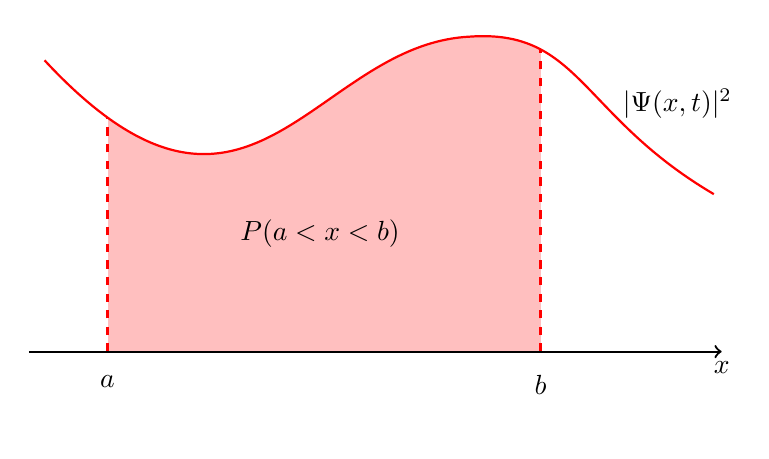
\begin{tikzpicture}
\begin{scope}
\clip (-0.3,3.7) .. controls (2.3,0.9) and (3.1,3.9) .. (5.1,4) .. controls (6.5,4.1) and (6.5,3) .. (8.2,2)--(6,-1)--(-.3,-1)--cycle;
\fill[pink] (0.5,0)node [below=5pt, black] {$a$}--(6,0)node [below=5pt, black] {$b$}--(6,5)--(0.5,5)--(0.5,0)--cycle ;
\draw[thick, red, dashed] (0.5,0)--(0.5,5);
\draw[thick, red, dashed] (6,0)--(6,5);
\node at (3.2,1.5) {$\Huge P(a<x<b)$};
\end{scope}
\draw[thick, red] (-0.3,3.7) .. controls (2.3,0.9) and (3.1,3.9) .. (5.1,4) .. controls (6.5,4.1) and (6.5,3) .. (8.2,2)node[black, above=15pt,pos=.9]{$|\Psi(x, t)|^2$};
\draw [thick, ->] (-.5,0)--(8.3,0) node[below]{$x$};
\end{tikzpicture}
\caption{\textit{Sannsynligheten for å finne en partikkel mellom $a$ og $b$.}}
\label{fig:prob}
\end{figure}

For at vi skal kunne tolke $|\Psi(x,t)|^2$ som en sannsynlighetstetthet må vi kreve at 
\begin{align}
	 \int_{-\infty}^{\infty} |\Psi(x,t)|^2 dx = 1
\end{align}
Vi trenger at bølgefunksjonen er \textbf{normaliserbar}, slik at vi kan tolke den 
probabilistisk. 
Fysikalsk kommer det av at partikkelen må nødvendigvis finnes et eller annet sted, og hvis 
vi integrerer over hele domenet (fra $-\infty$ til $\infty$) så må sannsynligheten være 1 
for at vi finner partikkelen.

Vi kan alltid normalisere bølgefunksjonen med mindre sannsynlighetstetthet divergerer for 
$|x|\to \infty$, hvis dette ikke er tilfellet kaller vi bølgefunksjonene \textbf{kvadrat integrerbar}. Dette krever vi at alle fysikalske bølegfunksjoner må være.


\subsection{Bevaring av sannsynlighet}
Vi skal nå se på om en bølgefunksjon som vi normaliserer ved et tidspunkt $t$ forblir
normalisert, altså om sannsynlighetstettheten er bevart i tid.

For å se på hvordan sannsynlighetstettheten endrer seg i tid beregner vi den tidsderiverte
\begin{align}
	 \frac{\partial |\Psi|^2}{\partial t} = \frac{\partial \Psi\Psi^*}{\partial t} =
	 \Psi^* \frac{\partial \Psi}{\partial t} + \Psi \frac{\partial \Psi^*}{\partial t} 
\end{align}
Vi har at vi kan skrive om S.L. slik at den gir oss 
\begin{align}
	 \frac{\partial \Psi}{\partial t} = \frac{1}{i\hbar}\Big(-\frac{\hbar^2}{2m}\frac{\partial^2 \Psi}{\partial x^2} + V(x)\Psi\Big) \end{align}
Vi antar at $V(x)$ er reelt og kompleks konjugerer denne ligningen 
\begin{align}
	 \frac{\partial \Psi^*}{\partial t} =
-\frac{1}{i\hbar}\Big(-\frac{\hbar^2}{2m}\frac{\partial^2\Psi^*}{\partial x^2}+V(x)\Psi^*\Big)
\end{align}
Vi bruker disse to ligningene og finner 
\begin{align} \label{eq:SL_cont}
	 \frac{\partial |\Psi|^2}{\partial t} &= i\frac{\hbar}{2m} \Big(\Psi^* 
  \frac{\partial^2 \Psi}{\partial x^2} - \Psi \frac{\partial^2 \Psi^*}{\partial x^2}\Big)\\
 &= \frac{\partial}{\partial x}\Big[  i\frac{\hbar}{2m} \Big(\Psi^* 
 \frac{\partial^2 \Psi}{\partial x} - \Psi \frac{\partial^2\Psi^*}{\partial x}\Big)\Big] 
\end{align}
Vi definerer nå \textbf{sannsynlighetsstrømmen} som 
\begin{align}
  j_x(x,t) = i\frac{\hbar}{2m} \Big(\Psi 
 \frac{\partial^2 \Psi^*}{\partial x} - \Psi^* \frac{\partial^2\Psi}{\partial x}\Big)
\end{align}
Dette gir 
\begin{align}
	 \frac{\partial |\Psi|^2}{\partial t} +\frac{\partial j_x(x,t)}{\partial x} = 0
\end{align}
Som er \textbf{kontinuitetsligningen} for sannsynlighetstettheten.
Dette er ekvivalent til kontinuitetsligningen fra elektrodynamikk som sier at ladningen 
må være bevart. Bevaring av ladning følger fra Maxwell's ligninger på samme måte 
som bevaring av sannsynlighet fra Schrödinger's ligning.

Videre har vi nå at 
\begin{align}
	 \frac{\partial}{\partial t} \int_{-\infty}^{\infty} |\Psi(x,t)|^2 dx =
 \int_{-\infty}^{\infty} \frac{\partial j_x(x,t)}{\partial x}  dx =
 \Big[-j_x(x,t)\Big]_{-\infty}^{\infty} = 0
\end{align}
hvor vi har brukt at $\Psi \to 0$ når $|x|\to \infty$, som vi vet behøves for at 
bølgefunksjonen skal være normaliserbar.

Hvis vi ser på hvordan sannsynligheten for en partikkel innenfor et interval $[a,b]$ 
endrer seg har vi 
\begin{align}
	 \frac{\partial }{\partial t} \int_{a}^{b} |\Psi(x,t)|^2 dx = \Big[ -j_x(x,t) \Big]
	= -j_x(b,t) + j_x(a,t)
\end{align}
Vi ser i Fig.~\ref{fig:j_x} et eksempel på hvordan sannsynlighetsstrømmen bestemmer endringen 
i sannsynlighetstetthet, og vi har fra kontinuitetsligningen at hvis sannsynlighetstettheten minker 
et sted, så dukker det ikke opp på et helt annet sted, men det flyter kontinuerlig mot at annet 
nærliggende område.
\begin{figure}[h!]
 \captionsetup{width=.8\linewidth}
\centering
\begin{tikzpicture}
%\fill[pink] (-1.,-1)--(1,-1)--(1,4)--(-1,4)--cycle ;
%\clip (-1.,1.2) .. controls (.2, 2.9) and (.7,1.2) .. (1.,2) -- (1, 4) -- (-1, 4);
%\draw[thick, black] (-1.,1.2) .. controls (.2, 2.9) and (.7,1.2) .. (1.,2);
\draw[blue,  thick, ->] (-3,2) -- (-1.1,2)  node[] at (-2, 2.75) {$j_x(a,t)>0$};
\draw[red,  thick, ->] (3,2) -- (1.1,2)  node[] at (2, 2.75) {$j_x(b,t)<0$};
\draw[red,  thick, <-] (-3,0) -- (-1.1,0)  node[] at (-2, 0.75) {$j_x(a,t)<0$};
\draw[blue,  thick, <-] (3,0) -- (1.1,0)  node[] at (2, 0.75) {$j_x(b,t)>0$};
\draw[black,  thick, ->] (-5,-1) -- (5,-1)  node[anchor=west]{$x$};
\filldraw[black] (1,-1) circle (1pt) node[anchor=north]{$b$};
\filldraw[black] (-1,-1) circle (1pt) node[anchor=north]{$a$};
\draw[gray, dashed, thick] (-1,-1) -- (-1,3);
\draw[gray, dashed, thick] (1,-1) -- (1,3);
\node[] at (0, 3.6) {$P(a<x<b)$} ;
\end{tikzpicture}
\caption{\textit{Sannsynlighetsstrømmen inn og ut av et område $[a,b]$ bestemmer hvordan 
sannsynlighetstettheten endrer seg på intervallet. Hvis e.g. $j_x(b,t)$ er negativ 
flyter sannsynlighetstrømmen inn i intervallet og det blir mer sannsynlig at partikkelen 
finnes der.
Tilsvarende hvis $j_x(a,t)$ er positiv, da flyter sannsynlighetstrømmen inn i $[a,b]$. 
Tidsutviklingen til sannsynligheten for å finne partikkelen i $[a,b]$ $P(a<x<b)$ er dermed gitt av 
sannsynlighetsstrommen.}}
\label{fig:j_x}
\end{figure}



\subsection{Forventningsverdier og uskarphet}
Forventnungsverdien til en måling av en partikkel med bølgefunksjon $\Psi(x,t)$ er 
\begin{align}
	 \langle x \rangle = \int_{-\infty}^{\infty} x |\psi(x,t)|^2 dx
\end{align}
hvor vi igjen antar at $|\Psi(x,t)|^2$ er normalisert. Forventningsverdien er ikke nødvendigvis 
den verdien vi burde forvente å måle, og kan i noen tilfeller til og med være en verdi 
som ikke er mulig å måle, men derimot gjennomsnittet av det man måler hvis man gjenntar 
eksperimentet mange ganger.
Videre har vi også at 
\begin{align}
	 \langle x^2 \rangle = \int_{-\infty}^{\infty} x^2 |\Psi(x,t)|^2 dx
\end{align}
Vi kan nå også se på standard avviket i posisjon til målingene, som vi har gitt som
\begin{align}
	 (\Delta x)^2 &=  \langle x - \langle x^2 \rangle \rangle \\
	 &=  \langle x^2 \rangle - \langle x \rangle^2 \\
	 &=  \int_{-\infty}^{\infty} x^2 |\Psi(x,t)|^2 dx 
	 -  \Big[\int_{-\infty}^{\infty} x |\psi(x,t)|^2 \Big]^2 dx
\end{align}
I kvantefysikk kaller vi $\Delta x$ uskarpheten i partikkelen's posisjon, som viser til 
en fundamental usikkerhet i bestemmelse av partikkelens possisjon siden partikkelen er beskrevet av bølgefunksjonen og den har ingen definitive posisjon.

Tilsvarende har vi for uskarpheten i bevegelsesmengde i x-retning
\begin{align}
	 (\Delta p_x)^2 =  \langle p_x^2 \rangle - \langle p_x \rangle^2 \\
\end{align}
Vi skal snart se hvordan vi beregner $\langle p_x \rangle$ fra bølgefunksjon i praksis.



\subsection{Ehrenfest's teorem}
Schrödinger's ligning er kvantemekanikken's bevegelsesligning, og kan brukes til å finne 
hvordan forventningsverdier utvikler seg i tid. 
Men vi vil at kvantefysikk spådommer er konsistent med klassisk fysikk i de riktige grensene 
(dette kalles noen ganger korrespondanseprinsippet).
Vi vet at i klassisk fysikk har vi 
\begin{align}
	 \frac{d x(t)}{d t} = \frac{p_x(t)}{m} 
\end{align}
Det betyr at vi burde ha 
\begin{align} \label{eq:ehrenfest}
     \frac{d\langle x \rangle}{dt} = \frac{\langle p_x \rangle}{m}	 
\end{align}
Vi skriver ut dette vha. definisjonen på forventningsverdi som 
\begin{align}
	\frac{d\langle x \rangle}{dt} &=  \frac{d}{dt} \int_{-\infty}^{\infty} x|\Psi(x,t)|^2 dx \\
				      &=  \int_{-\infty}^{\infty} x \frac{d\Psi\Psi^*}{dt}dx\\
		&=   \int_{-\infty}^{\infty} x \frac{\partial}{\partial x} \Big( \frac{i\hbar}{2m} 
     (\Psi^*  \frac{\partial \Psi}{\partial x} - \Psi \frac{\partial \Psi^*}{\partial x})\Big)dx 
\end{align}
hvor vi har brukt Lign.~[\ref{eq:SL_cont}]; S.L. multiplisert med den kompleks konjugerte
av bølgefunksjonen. Vi kan løse dette ved hjelp av delvis integrasjon
\begin{align}
\frac{d\langle x \rangle}{dt} &=
  - \int_{-\infty}^{\infty}  \frac{i\hbar}{2m} 
  (\Psi^*  \frac{\partial \Psi}{\partial x} - \Psi \frac{\partial \Psi^*}{\partial x})dx  +
  \Big[x \frac{\partial}{\partial x} \Big( \frac{i\hbar}{2m} 
 (\Psi^*\frac{\partial \Psi}{\partial x} - \Psi \frac{\partial \Psi^*}{\partial x})\Big)
  \Big]_{-\infty}^{\infty} \\ 
 &=-\int_{-\infty}^{\infty}  \frac{i\hbar}{2m} 
  (\Psi^*  \frac{\partial \Psi}{\partial x} - \Psi \frac{\partial \Psi^*}{\partial x})dx  \\
 &=-\int_{-\infty}^{\infty}  \frac{i\hbar}{2m} 
  (\Psi^*  \frac{\partial \Psi}{\partial x} + \Psi^* \frac{\partial \Psi}{\partial x})dx  \\
 &=-\int_{-\infty}^{\infty}  \frac{i\hbar}{m} \Psi^*  \frac{\partial \Psi}{\partial x}dx \\
 &= \frac{1}{m} \int_{-\infty}^{\infty} \Psi^*\frac{\hbar}{i}\frac{\partial \Psi}{\partial x}dx
\end{align}
Vi kan sammenligne dette med Lign.~[\ref{eq:ehrenfest}] og vi ser at vi da har 
\begin{align}
	\langle p_x \rangle 
	= \int_{-\infty}^{\infty}\Psi^*\frac{\hbar}{i}\frac{\partial \Psi}{\partial x}dx
\end{align}
Hvor vi nå også har en måte å finne forventningsverdien til bevegelsesmengden.

Vi har også i klassisk fysikk at 
\begin{align}
	F = \frac{\partial p_x}{\partial t} = - V'(x)
\end{align}
Hvilket betyr at vi også skulle forvente etter korrespondanseprinsippet å ha i kvantefysikken
\begin{align}
	 \frac{d \langle p_x \rangle }{d t} = - \big\langle \frac{d V}{d x}  \big\rangle
\end{align}
Dette og Lign.~[\ref{eq:ehrenfest}] kaller vi \textbf{Ehrenfest's teorem}. Selv om det strengt tatt bare 
er to spesiall tilfeller av et mer generelt teorem. 

\subsection{Kvalitativt om Heisenberg's uskarphetsrelasjon}

\begin{figure}[h!]
     \centering
     \begin{subfigure}[b]{0.3\textwidth}
       \centering
	\begin{tikzpicture}[width=\textwidth]
	  \begin{axis}%
	    [grid=both,
	     minor tick num=1,
	     xlabel=$x$,
	     ylabel=$y$,
	     grid style={line width=.01pt, draw=gray!10},
	     major grid style={line width=.2pt,draw=gray!50},
	     axis lines=middle,
	     restrict y to domain=-1:1.,
	     enlargelimits={abs=1.25}
	    ]
	    \addplot+[mark=none, 
		    domain=-4:4,
		    samples=150,
		    hatch distance=5pt,
		    hatch thickness=0.5pt,
		    draw=blue!70,
		    pattern color=blue,
		    area legend] {cos(deg(pi*x))}  node[pos=0] (endofplot_1) {};
	    \node [above, color=blue!70] at (endofplot_1) {$\cos(kx)$};
	  \end{axis}
	\end{tikzpicture}
         \caption{$y=\cos(kx) $}
         \label{fig:cos}
     \end{subfigure}
     \hspace{3cm}
     \begin{subfigure}[b]{0.3\textwidth}
         \centering
	\begin{tikzpicture}[width=\textwidth]
	\begin{axis}%
	[grid=both,
	minor tick num=1,
	xlabel=$x$,
	ylabel=$y$,
	grid style={line width=.01pt, draw=gray!10},
	major grid style={line width=.2pt,draw=gray!50},
	axis lines=middle,
	restrict y to domain=-4:4.,
	enlargelimits={abs=.25}
	]
	\addplot+[mark=none, 
	    domain=-5:35,
	    samples=350,
	    hatch distance=5pt,
	    hatch thickness=0.5pt,
	    draw=red!70,
	    pattern color=blue,
	    %area legend] {cos(deg(2*pi*x)) / (1 + (x - 20)^2)}  ;
	    area legend] {1 / (1 + 0.1*(x - 20)^2)}  ;
  \node[above, color=red!70] at (8, 0.25) {$\frac{1}{1+(x-25)^2}$};
	\end{axis}
	\end{tikzpicture}
         \caption{Kort bølge-puls}
         \label{fig:puls}
     \end{subfigure}
        \caption{Cosinus kurven har en bestemt og lett målbar bølgelengde, men vi kan ikke 
	bestemme posisjonen til kurven. Den korte puls-kurven derimot har en skarpt bestemt 
	posisjon men ingen definert bølgelengde.
	Det hinter mot en trade-off mellom å bestemme bølgelengde og posisjon.}
        \label{fig:bølger}
\end{figure}
Hvis vi ser for oss to vannbølger som i Fig.~\ref{fig:bølger} som brer seg over vannet.
Når vi har en cosinus eller sinus kurve som i Fig.~\ref{fig:cos} 
så kan vi lett måle bølgens bølgelengde men ikke hvor bølgen er; bølgen er over 
alt og det er umulig å bestemme dens posisjon til et punkt i rommet. 
Hvis vi på den andre siden ser for oss en kort bølge-puls som i Fig.~\ref{fig:puls}
så er det lett å måle hvor den befinner seg i rommet, men ikke bølgelengden.

Hvis vi ser for oss lydbølger, har vi da at en ren tone er en ren sinuskurve, mens et klapp er en 
kort puls som dør ut veldig fort siden hendene våre ikke gir resonans. Vi vet at man lett kan 
høre tonehøyden til en ren tone og høre forskjell på forskjellige rene toner, men selv ikke 
trente musikere kan høre tonehøyden til ett klapp. Dette kommer av at lydbølgene dør så fort at 
man ikke kan bestemme frekvensen, i motsetning til den rene tonen som består av bølge som svinger
over lengre tid. Så vi har da at jo lengre lydbølgen svinger jo bedre kan vi bestemme frekvensene
den består av.

Begge de to nevnte eksemplene kan forklares ved Fourier-teori, hvor vi har at alle (eller 
i hvert fall de aller fleste) funksjoner kan dekomponeres som en sum av sinus og cosinus kurver.
Vi har da funksjon $f(x)$ definert på et intervall av lengde $L$ kan approkismeres arbitrært godt med 
\begin{align}
	 f_N(x) = \frac{a_0}{2} \sum_{n=-N}^{N} \Big( a_n \cos(\frac{2\pi}{L} nx ) +
	b_n \sin(\frac{2\pi}{L} nx )     \Big)
\end{align}

Dvs. at det tyder på at vi enten kan bestemme bølgelengde skarpt eller vi kan bestemme posisjonen
skarpt. Vi kan også trekke denne analogen til partikler også, hvor vi da ikke kan bestemme 
bølgelengde og posisjon skarpt samtidig. 
Siden vi vet at bevegelsesmengden til en partikkel i kvantemekanikken er 
gitt ved  $p=\frac{h}{\lambda}$ har vi da at bevegelsesmengden ikke kan bestemmes skarpt. 
Dette leder til Heisenberg's berømte uskarphetsrelasjon som sier at vi ikke kan bestemme  
posisjon og bevegelsesmengde helt nøyaktig samtidig. Dette gjelder på sett og vis 
også for energi og tid.

Generelt har vi at hvis noe er skarpt lokalisert i $k$ så er det mindre lokalisert i $x$. 
Man kan vise utifra Fourier-teori at
\begin{align}
	 \Delta x \Delta k \ge \frac{1}{2}
\end{align}
Når vi bruker at $p=\hbar k$, gir dette oss \textbf{Heisenberg's uskarphetsrelasjon}
\begin{align}
	 \Delta x \Delta k \ge \frac{\hbar}{2}
\end{align}



Dette er dog ikke et kvantefenomem, men et helt generelt fenomen som gjelder for all 
bølgebevegelse, de rare konsekvensene vi får ifra uskarphetsrelasjonen er bare et resultat 
av at vi beskriver partikler som sannsynlighetsbølger i kvantefysikken.

Vi har sett at planbølger på formen 
\begin{align}
	 \Psi(x,t) = Ce^{i(kx - \omega t)}
\end{align}
er løsninger til S.L., men vi ser fort at dette er problematisk siden vi har sagt at bare kvadrat 
integrerbare bølgefunksjoner er fysikalske. Vi ser at planbølger ikke er kvadrat integrerbar og
ikke kan normaliseres siden de ikke går mot 0 når $|x| \to \infty$ som vi ser i Fig.~\ref{fig:non_norm}. 
I tillegg kan vi ikke bestemme posisjonen til en planbølge siden den er overalt i rommet, 
og vi ønsker å kunne betrakte lokaliserte partikler.

Men vi vet at S.L. er lineær og hvis vi har to løsninger av S.L. så er lineær kombinasjon av de 
også en løsning. Vi kan overlagre bølger og skape noe som er mer lokalisert i rommet, som vi ser 
antydninger til i Fig.~\ref{fig:superposition}. Vi har at for 4 overlagrede bølger kan vi skape en 
ganske lokalisert puls, men som gjentas i det uendelige.
\begin{figure}[h!]
     \centering
     \begin{subfigure}[b]{0.8\textwidth}
       \centering
	\begin{tikzpicture}[width=\textwidth]
	  \begin{axis}%
	    [grid=both,
	     minor tick num=1,
	     xlabel=$x$,
	     ylabel=$y$,
	     grid style={line width=.01pt, draw=gray!10},
	     major grid style={line width=.2pt,draw=gray!50},
	     axis lines=middle,
	     restrict y to domain=-1:1.,
	     enlargelimits={abs=1.25}
	    ]
	    \addplot+[mark=none, 
		    domain=-4:4,
		    samples=150,
		    hatch distance=5pt,
		    hatch thickness=0.5pt,
		    draw=red!70,
		    pattern color=blue,
		    area legend] {cos(deg(pi*x))}  node[pos=1] (endofplot) {};
	    \node [above, color=red!70] at (endofplot) {$\cos(kx)$};
	    \addplot+[mark=none, 
		    domain=-4:4,
		    samples=150,
		    hatch distance=5pt,
		    hatch thickness=0.5pt,
		    draw=blue!70,
		    pattern color=blue,
		    area legend] {cos(deg(pi*x))^2}  node[pos=0] (endofplot_1) {};
	    \node [above, color=blue!70] at (endofplot_1) {$\cos^2(kx)$};
	  \end{axis}
	\end{tikzpicture}
         \caption{$y=\cos(kx)$ og $y' = \cos^2(kx)$}
         \label{fig:non_norm}
     \end{subfigure}
     \hspace{4cm}
     \begin{subfigure}[b]{0.3\textwidth}
         \centering
	\begin{tikzpicture}[width=\textwidth]
	  \begin{axis}%
	    [grid=both,
	     minor tick num=1,
	     xlabel=$x$,
	     ylabel=$y$,
	     grid style={line width=.01pt, draw=gray!10},
	     major grid style={line width=.2pt,draw=gray!50},
	     axis lines=middle,
	     restrict y to domain=-2:2.,
	     enlargelimits={abs=2.}
	    ]
	    \addplot+[mark=none, 
		    domain=-35:35,
		    samples=350,
		    hatch distance=5pt,
		    hatch thickness=0.5pt,
		    draw=red!70,
		    pattern color=blue,
		    area legend] {cos(deg((pi + .4)*x)) + cos(deg(pi*x))} ;
	    \node [below, color=red!70] at (20, -2) {$\cos(kx) + \cos(k'x)$};
	  \end{axis}
	\end{tikzpicture}
         \caption{$y=\cos(kx) + \cos(k'x)$}
         \label{fig:2super}
     \end{subfigure}
     \hspace{3cm}
     \begin{subfigure}[b]{0.3\textwidth}
         \centering
	\begin{tikzpicture}[width=\textwidth]
	\begin{axis}%
	[grid=both,
	minor tick num=1,
	xlabel=$x$,
	ylabel=$y$,
	grid style={line width=.01pt, draw=gray!10},
	major grid style={line width=.2pt,draw=gray!50},
	axis lines=middle,
	restrict y to domain=-4:4.,
	enlargelimits={abs=2.}
	]
	\addplot+[mark=none, 
	    domain=-35:35,
	    samples=350,
	    hatch distance=5pt,
	    hatch thickness=0.5pt,
	    draw=red!70,
	    pattern color=blue,
	    area legend] {cos(deg((pi + .2)*x)) + cos(deg(pi*x)) +
			  cos(deg((pi + .4)*x)) + cos(deg((pi + 0.6)*x))} ;
	\node [below, color=red!70] at (1, -4) {$\cos(kx) + \cos(k'x)  + \cos(k''x) + \cos(k'''x)$};
	\end{axis}
	\end{tikzpicture}
         \caption{$y=\cos(kx) + \cos(k'x) + \cos(k''x) + \cos(k'''x)$}
         \label{fig:4super}
     \end{subfigure}
        \caption{Ovelagring av cosinus bølger.}
        \label{fig:superposition}
\end{figure}
Hvis vi overlagrer uendelig mange bølge kan vi skape en puls som gjentas uendelig sjelden, dvs som er 
lokalisert rundt ett området i rommet. 
Siden vi trenger uendelig mange overlagrede bølger blir summen vår til et integral, og vi har 
\begin{align}
	 \Psi(x,t) = \int_{-\infty}^{\infty} A(k)e^{i(kx - \omega(k) t)} dk
\end{align}
hvor vi inkluderer alle mulige bølgelengder ved at vi integrerer over $k$. Dette er nå noe som kan være 
lokalisert, gitt at $A(k)$ er det. 

\subsubsection{Gaussisk Bølgepakke}
Vi skal nå se på en Gaussisk bølgepakke, hvor vi lar $A(k)$ ha formen til en Gauss-kurve, vi har da 
\begin{align}
   A(k) = \frac{\sqrt{\sigma}}{\sqrt{2\pi}\pi^{\frac{1}{4}} } e^{-(k-k_0)^2 \frac{\sigma^2}{2}}
\end{align}
hvor $\sigma$ er bredden til Gauss-kurven og $k_0$ bølgetallet som kurven er sentrert rundt. 
Vi har nå følgende bølgefunksjon
\begin{align}
	 \Psi(x, t) = \frac{\sqrt{\sigma}}{\sqrt{2\pi}\pi^{\frac{1}{4}} } \int_{-\infty}^{\infty} 
	e^{-(k-k_0)^2 \frac{\sigma^2}{2}} e^{i(kx - \omega(k)t)} dk
\end{align}
Dette tilfredstiller S.L. siden vi vet at S.L. er lineær og vi har har en sum 
linearkombinasjon av løsninger til S.L. (et integral, men som vi kan se på 
som en kontinuerlig sum).
\begin{figure}[h!]
     \centering
	\begin{tikzpicture}[width=\textwidth]
	\begin{axis}%
	[grid=both,
	minor tick num=1,
	xlabel=$k$,
	ylabel=$A(k)$,
	grid style={line width=.01pt, draw=gray!10},
	major grid style={line width=.2pt,draw=gray!50},
	axis lines=middle,
	restrict y to domain=-5:5.,
	enlargelimits={abs=.2}
	]
	\addplot+[mark=none, 
	    domain=0:4,
	    samples=350,
	    hatch distance=5pt,
	    hatch thickness=0.5pt,
	    draw=red!70,
	    pattern color=blue,
	    area legend] {exp(-(2-x)^2 / (2*0.25^2)) / (0.25 * sqrt(pi))  } ;
	\node [below, color=red!70] at (2.6, 2) {$A(k)$};
	\end{axis}
	\end{tikzpicture}
        \caption{Gauss-kurve}
        \label{fig:superposition}
\end{figure}
Vi skal nå finne et eksplisitt uttrykk for denne bølgefunksjon. Vi starter med å se på den 
tidsuavhengige delen av bølgefunksjonen dvs. vi betrakter 
\begin{align}
	 \psi(x) = \Psi(x, 0) = \frac{\sqrt{\sigma}}{\sqrt{2\pi}\pi^{\frac{1}{4}} } 
	\int_{-\infty}^{\infty} e^{-(k-k_0)^2 \frac{\sigma^2}{2}} e^{ikx} dk
\end{align}
Vi kan beregne $\psi(x)$ ved å regne integralet. For å gjøre det skriver vi om eksponenten
slik at vi får et uttrykk som er lettere å jobbe med. Vi får da 
\begin{align}
   -(k-k_0)^2 \frac{\sigma^2}{2} + ikx
&= -\frac{\sigma^2}{2} \Big[k^2 - 2kk_0 + k_0^2\Big] + \frac{\sigma^2}{2} ikx \frac{2}{\sigma^2} \\
&= -\frac{\sigma^2}{2} \Big[k^2 - 2kk_0 - ikx\frac{2}{\sigma^2}\Big] - k_0^2  \frac{\sigma^2}{2} \\
&= -\frac{\sigma^2}{2} \Big[k^2- 2k(k_0-\frac{ix}{\sigma^2}) + (k_0 + \frac{ix}{\sigma^2})^2\Big] 
   + \frac{\sigma^2}{2} (k_0 + \frac{ix}{\sigma^2})^2 - k_0^2  \frac{\sigma^2}{2} \\
   &= -\frac{\sigma^2}{2} \Big[k  - (k_0 + \frac{ix}{\sigma^2})\Big]^2 
   + \frac{\sigma^2}{2} (k_0 + \frac{ix}{\sigma^2})^2 - k_0^2  \frac{\sigma^2}{2} \\
   &= -\frac{\sigma^2}{2} \Big[k  - k_0 - \frac{ix}{\sigma^2}\Big]^2 
   + \frac{\sigma^2}{2} (k_0^2 + 2k_0\frac{ix}{\sigma^2} + (\frac{ix}{\sigma^2})^2) - 
   k_0^2  \frac{\sigma^2}{2} \\ 
   &= -\frac{\sigma^2}{2} \Big[k  - k_0 - \frac{ix}{\sigma^2}\Big]^2 
   + \frac{\sigma^2}{2} ( 2k_0\frac{ix}{\sigma^2} + (\frac{ix}{\sigma^2})^2)  \\ 
   &= -\frac{\sigma^2}{2} \Big[k  - k_0 - \frac{ix}{\sigma^2}\Big]^2 
   + ik_0x - \frac{x^2}{2\sigma^2}
\end{align}
Vi kan nå skrive uttrykket for bølgefunksjonen som 
\begin{align}
	 \psi(x) &= \frac{\sqrt{\sigma}}{\sqrt{2\pi}\pi^{\frac{1}{4}} } 
	\int_{-\infty}^{\infty} e^{-\frac{\sigma^2}{2}(k - k_0 - \frac{ix}{\sigma^2})^2} 
	e^{ik_0x} e^{-\frac{x^2}{2\sigma^2}} dk \\
&= \frac{\sqrt{\sigma}}{\sqrt{2\pi}\pi^{\frac{1}{4}} } e^{ik_0x} e^{-\frac{x^2}{2\sigma^2}}
	\int_{-\infty}^{\infty} e^{-\frac{\sigma^2}{2}(k - k_0 - \frac{ix}{\sigma^2})^2} dk
\end{align}
Vi kan nå beregne integralet og finne bølgefunksjonen. Vi trenger et kjent integral 
\begin{align}
	 I = \int_{-\infty}^{\infty} e^{(x - i\lambda)^2} dx = \sqrt{\pi} 
\end{align}
og vi utfører et variabelskifte og setter 
\begin{align}
	 y &= \frac{\sigma}{\sqrt{2}}(k-k_0) \\
	\frac{d y}{d k} &= \frac{\sigma}{\sqrt{2}} \\
	d k &= \frac{\sqrt{2}}{\sigma} d y
\end{align}
Dette gir 
\begin{align}
	 \psi(x) &= \frac{\sqrt{\sigma}}{\sqrt{2\pi}\pi^{\frac{1}{4}} } 
	e^{ik_0x} e^{-\frac{x^2}{2\sigma^2}} 
	\int_{-\infty}^{\infty} e^{-(y - \frac{ix}{\sqrt{2}\sigma})^2} \frac{\sqrt{2}}{\sigma}dy\\
	 &= \frac{1}{\sqrt{\sigma}\pi^{\frac{1}{4}} } 
	e^{ik_0x} e^{-\frac{x^2}{2\sigma^2}} 
\end{align}
\begin{figure}[h!]
     \centering
	\begin{tikzpicture}[width=\textwidth]
	\begin{axis}%
	[grid=both,
	minor tick num=1,
	xlabel=$x$,
	ylabel=$y$,
	grid style={line width=.01pt, draw=gray!10},
	major grid style={line width=.2pt,draw=gray!50},
	axis lines=middle,
	restrict y to domain=-5:5.,
	enlargelimits={abs=.2}
	]
	\addplot+[mark=none, 
	    domain=-2:2,
	    samples=350,
	    hatch distance=5pt,
	    hatch thickness=0.5pt,
	    draw=blue!70,
	    pattern color=blue,
	    area legend] {exp(-x^2 / (2*0.25^2)) * cos(deg(20*x) / (0.25 * sqrt(pi))  } ;
	\node [below, color=blue!70] at (1.6, 1) {$\mathcal{R} \{ \psi(x) \}$};
	\addplot+[mark=none, 
	    domain=-2:2,
	    samples=350,
	    hatch distance=5pt,
	    hatch thickness=0.5pt,
	    draw=red!70,
	    pattern color=blue,
	    area legend] {exp(-x^2 / (2*0.25^2)) / (0.25 * sqrt(pi))  } ;
	\node [below, color=red!70] at (1.6, 2) {$|\psi(x)|^2$};
	\end{axis}
	\end{tikzpicture}
        \caption{Bølgefunksjonen til Gaussisk bølgepakke}
        \label{fig:gaussian_x}
\end{figure}
Vi har altså vist at både $A(k)$ og $|\psi(x)|^2$ er Gauss-kurver, hvilket kommer av at 
Gauss-funksjonen er invariant under Fourier-transformasjon. 

Vi kan nå se på uskarpheten for bølgepakken. Vi starter med posisjonen
\begin{align}
    \langle x \rangle &= \frac{1}{\sqrt{\pi}\sigma } \int_{-\infty}^{\infty} x 
                     e^{-\frac{x^2}{\sigma^2}} dx \\
         &= 0
\end{align}
hvor vi har brukt at integranden er asymmetrisk, siden $x$ er asymmetrisk og 
$e^{ \frac{x^2}{\sigma^2}}$ er symmetriks på et symmetrisk intervall om $0$.
Videre har vi 
\begin{align}
    \langle x^2 \rangle &= \frac{1}{\sqrt{\pi}\sigma } \int_{-\infty}^{\infty} x^2 
                     e^{-\frac{x^2}{\sigma^2}} dx \\
         &= \frac{1}{\sqrt{\pi}\sigma }  \frac{\sqrt{\pi} \sigma^{3}}{2} \\
         &=  \frac{\sigma^{2}}{2}
\end{align}
Hvor vi brukte det kjente integralet 
\begin{align}
	 \int_{-\infty}^{\infty} x^2 e^{-\beta x^2}dx = \frac{\sqrt{\pi} \beta^{-\frac{3}{2}}}{2}
\end{align}
Vi regner nå ut forventningsverdien til bevegelsesmengden som vi vet hvordan man 
beregner takket være Ehrenfest's teorem
\begin{align}
\langle p \rangle &= \frac{1}{\sqrt{\pi}\sigma } \int_{-\infty}^{\infty}e^{-\frac{x^2}{2\sigma^2}}
  \Big(\frac{\hbar}{i}\frac{\partial }{\partial x} \Big) e^{-\frac{x^2}{2\sigma^2}} dx \\
 &= \frac{i\hbar}{\sqrt{\pi}\sigma } \int_{-\infty}^{\infty}e^{-\frac{x^2}{2\sigma^2}}
   \frac{x}{\sigma^2} e^{-\frac{x^2}{2\sigma^2}} dx \\
 &= \frac{i\hbar}{\sqrt{\pi}\sigma^3 } \int_{-\infty}^{\infty} x e^{-\frac{x^2}{\sigma^2}} dx \\
 &= 0
\end{align}
Til sist beregner vi 
\begin{align}
\langle p^2\rangle &= \frac{1}{\sqrt{\pi}\sigma} \int_{-\infty}^{\infty}e^{-\frac{x^2}{2\sigma^2}}
  \Big(\frac{\hbar}{i}\frac{\partial }{\partial x} \Big)^2 e^{-\frac{x^2}{2\sigma^2}} dx \\
 &= \frac{\hbar^2}{\sqrt{\pi}\sigma } \int_{-\infty}^{\infty}e^{-\frac{x^2}{2\sigma^2}}
  \frac{\partial }{\partial x} \big( \frac{x}{2\sigma^2} e^{-\frac{x^2}{2\sigma^2}} \Big) dx \\
 &= \frac{\hbar^2}{2\sqrt{\pi}\sigma^3 } \int_{-\infty}^{\infty}e^{-\frac{x^2}{2\sigma^2}}
  \Big(1 + \frac{x}{2\sigma^2} \Big)e^{-\frac{x^2}{2\sigma^2}} dx \\
 &= \frac{\hbar^2}{2\sqrt{\pi}\sigma^3 } \int_{-\infty}^{\infty}e^{-\frac{x^2}{\sigma^2}}dx \\
 &= \frac{\hbar^2}{2\sqrt{\pi}\sigma^3 } \sigma \int_{-\infty}^{\infty}e^{-x'^2}dx' \\
 &= \frac{\hbar^2}{2\sigma^2 } 
\end{align}
Vi har at 
\begin{align}
	(\Delta x)^2 (\Delta p)^2 &= (\langle p^2\rangle - \langle p\rangle^2)
   (\langle x^2\rangle -\langle x\rangle^2 ) \\
   &= \frac{\hbar^2}{4}
\end{align}
Dvs. vi har funnet at bølgepakken er helt på grensen av det som er tillatt ved Heisenberg's 
uskarphetsrelasjon. Bølgepakken er maksimalt uskarp, siden vi har
\begin{align}
	\Delta x\Delta p = \frac{\hbar}{2}
\end{align}


\subsubsection{Tidsavhengig Gaussisk bølgefunksjon}
Vi skal nå finne den tidsavhengige bølgefunksjon
\begin{align}
	 \Psi(x, t) = \frac{\sqrt{\sigma}}{\sqrt{2\pi^{\frac{3}{2}}}}  
	\int_{-\infty}^{\infty} e^{-(k-k_0)^2\frac{\sigma^2}{2}}
	e^{i(kx - \omega t)} dx
\end{align}
hvor vi da må løse det litt vriene integralet. Vi skal gjøre dette ved å først vise at vi kan skrive det om til
\begin{align}
	 \Psi(x, t) = \frac{\sqrt{\sigma}}{\sqrt{2\pi^{\frac{3}{2}}}} e^{i(k_0 x - \omega_0 t)} 
	\int_{-\infty}^{\infty} e^{-(k-k_0)^2(\frac{\sigma^2}{2} + \frac{it\hbar}{2m})}
	e^{i(k-k_0)(x - \frac{k_0\hbar t}{m})} dx
\end{align}
Vi bruker at $\omega = \hbar k^2 / 2m$ og kan vise at eksponentene i de to uttrykkene er 
ekvivalente
\begin{align}
	 & i(k_0 - \omega_0) - (k - k_0)^2(\frac{\sigma^2}{2} + \frac{it\hbar}{2m}) + i(k-k_0)(x - \frac{k_0\hbar t}{m}) \\
	= & i(k_0x - \omega_0t) - k^2  \frac{it\hbar}{2m} + 2kk_0 \frac{it\hbar}{2m} - k_0^2 \frac{it\hbar}{2m} - (k-k_0)^2\frac{\sigma^2}{2} + i(k-k_0)x - \frac{ik k_0 \hbar t}{m} + \frac{ik_0^2 \hbar t}{m}	 \\ 
	= & i(k_0x - \omega_0t) - i\omega t + 2kk_0 \frac{it\hbar}{2m} - i\omega_0 t - (k-k_0)^2\frac{\sigma^2}{2} + i(k-k_0)x - \frac{ik k_0 \hbar t}{m}  + 2i\omega_0 t \\ 
	= & -(k-k_0)^2\frac{\sigma^2}{2} + i(kx-\omega t) 
\end{align}
Som er det vi ville vise. Videre gjøre vi de følgende variabel-substitusjonene
\begin{align}
	 y &= k - k_0 \\ 
	a &= \frac{1}{\sqrt{\frac{\sigma^2}{2} + \frac{i\hbar t}{2m}}}  \\ 
	 b &= x - \frac{k_0 \hbar t}{m}
\end{align}
som gir oss
\begin{align}
	 \Psi(x,t) = \frac{\sqrt{\sigma} }{\sqrt{2\pi^{\frac{3}{2}}} } e^{i(k_0x - \omega_0t)} 
	\int_{-\infty}^{\infty} e^{-(\frac{y}{a})^2}e^{iyb}dy
\end{align}
Vi kan nå utnytte det følgende kjente integral
\begin{align}
	 \int_{-\infty}^{\infty} e^{-(x - i \Lambda)^2} dx = \sqrt{\pi} 
\end{align}
Vi kan da bruke dette resultatet og introdusere en ny variabel $y=ax$ og definere en ny konstant
$b = \frac{2\Lambda}{a}$. Dette gir da
\begin{align}
	\int_{-\infty}^{\infty} e^{-(x - i \Lambda)^2} dx
	&= \int_{-\infty}^{\infty} e^{-x^2 + \Lambda^2 + 2 x i \Lambda} dx \\
	&= e^{\Lambda^2} \int_{-\infty}^{\infty} e^{-x^2  + 2 x i \Lambda} dx \\
	&= e^{\frac{a b }{2}} a^{-1} \int_{-\infty}^{\infty} e^{-(\frac{y}{a})^2  +  ib y  } dy  \\
	&= \sqrt{\pi} 
\end{align}
Vi inverterer dette uttrykket og får
\begin{align}
	\sqrt{\pi} a e^{-(\frac{ab}{2})^2} =  \int_{-\infty}^{\infty} e^{-(\frac{y}{a})^2 + iby}dy 
\end{align}
Vi bruker nå at vi har at
\begin{align}
	 \big(\frac{ab}{2}\big)^2 = \big(\frac{1}{2}\frac{x - \frac{k_0 \hbar t}{m}}{\sqrt{\frac{\sigma ^2}{2} + \frac{i \hbar t}{2m}} }\big)^2
\end{align}
og vi har nå funnet uttrykket for den tidsavhengige bølgefunksjon
\begin{align}
	 \Psi(x,t) &= \frac{\sqrt{\sigma}}{\sqrt{2}\pi^{\frac{3}{2}}} e^{i(k_0x - \omega_0 t)} \sqrt{\pi}
	\frac{1}{\sqrt{\frac{\sigma ^2}{2} + 
	\frac{i\hbar t}{2m}} }e^{-\frac{1}{4}\frac{(x-\frac{k_0 \hbar t}{m})^2}{\frac{\sigma^2}{2} + \frac{i\hbar t}{2m}} } \\ 
	&= \frac{\sqrt{\sigma}}{\sqrt{\sigma ^2 + \frac{i\hbar t}{m}} \sqrt{\pi}} 
	e^{i(k_0x - \omega_0 t)} e^{-\frac{1}{2}\frac{(x-\frac{k_0 \hbar t}{m})^2}{\sigma^2 + \frac{i\hbar t}{m}}}
\end{align}
Vi kan også finne absolutt kvadratet
\begin{align}
  |\Psi(x,t)|^2 &= \frac{\sigma}{\sqrt{(\sigma^2 +
  	\frac{i\hbar t}{m})(\sigma^2-\frac{i\hbar t}{m})} \sqrt{\pi}} 
	e^{-\frac{1}{2}\frac{(x-\frac{k_0 \hbar t}{m})^2}{\sigma^2 + \frac{i\hbar t}{m}}}  
	e^{-\frac{1}{2}\frac{(x-\frac{k_0 \hbar t}{m})^2}{\sigma^2 - \frac{i\hbar t}{m}}} \\ 
&= \frac{1}{\sqrt{\sigma^4 + \frac{\hbar t^2}{\sigma^2m^2}} \sqrt{\pi}} 
	e^{-\frac{(x-\frac{k_0 \hbar t}{m})^2}{\sigma^2 + \frac{\hbar^2 t^2}{\sigma^2m^2}}}  
\end{align}
Vi ser at vi som forventet har at 
\begin{align}
	 |\Psi(x, t=0)|^2 = \frac{1}{\sqrt{\pi} \sigma}e^{-\frac{x^2}{\sigma^2}}
\end{align}
Ved tid $t=0$ er den tidsavhegige bølgepakken lik den stasjonære. 
Uskarpheten må derfor også være den samme ved $t=0$
\begin{align}
	 \Delta x(t=0)^2 = \frac{\hbar}{2}
\end{align}
Vi kan finne hvordan uskarpheten utvikler seg i tid ved hjelp av standard formler for definisjonen
av uskarphet, dvs. ed å beregne forventningsverdiene for $x$, $x^2$, $p$ og $p^2$.
Men vi kan også se på hvordan uttrykkene forandrer seg fra stasjonær til tidsavhengig bølgepakke,
hvor vi essensialt gjør følgende variabel-bytte
\begin{align}
	 \sigma^2 \to  \sigma^2 + \frac{\hbar^2 t^2}{\sigma^2 m^2}
\end{align}
Altså må uskarpheten være
\begin{align}
	 \Delta x(t) = \frac{1}{\sqrt{2}} \sqrt{\sigma^2 + \frac{\hbar^2t^2}{\sigma^2 m^2}}  
\end{align}
Uskarpheten i bevegelsesmengde hadde vi opprinnelig som 
\begin{align}
	 \Delta p(t=0)^2 = \frac{\hbar}{\sqrt{2} \sigma}
\end{align}
og hvis vi ser på bølgepakken in bevegelsesmengde-rommet
\begin{align}
	 \Psi(x, t) = \frac{\sqrt{\sigma}}{\sqrt{2\pi^{\frac{3}{2}}}}  
	\int_{-\infty}^{\infty} e^{-(k-k_0)^2\frac{\sigma^2}{2}}
	e^{i(kx - \omega t)} dk
\end{align}
ser vi at den delen av bølgefunksjonen som gir bredden til bølgepakken er invariant i tid. 
Derfor må det holde at uskarpheten i bevegelsesmengde er lik for alle tider, slik som den var 
for $t=0$
\begin{align}
	 \Delta p(t)^2 = \frac{\hbar}{\sqrt{2} \sigma}
\end{align}
Vi har nå funnet at tidsutviklingen til uskarpheten til en Gaussisk bølgepakke er
\begin{align}
	 \Delta p(t)  \Delta x(t) = \frac{\hbar}{2}\sqrt{1 + \frac{\hbar^2 t^2}{\sigma^{4}m^2}} 
\end{align}


\subsection{Fase og gruppe-hastighet}
Vi vet at vi har farten til en planbølge gitt ved 
\begin{align}
	 v_f = \frac{dx}{dt}
\end{align}
Dette kaller vi fasehastigheten, farten som en bølgetopp beveger seg med.
Siden vi har $kdx - \omega dt = 0$ 
når vi følger en bølgetopp (vi er hele tiden på samme punktet i bølgen), har vi
\begin{align}
	 v_{f} = \frac{\omega}{k} = \lambda \nu 
\end{align}
Men dette beskriver ikke hastigheten til en ikke-relativistisk partikkel, som vi kan se ifra S.L.
siden vi har at 
\begin{align}
	v_f = \frac{\omega}{k} = \frac{\hbar\omega}{\hbar k} = \frac{E}{p} 
	= \frac{\frac{mv^2}{2}}{mv} = \frac{v}{2}
\end{align}
Vi har argumentert for at bølgepakken er det som beskriver en fri partikkel og 
siden vi har at bølgepakken er en uendelig sum av planbølger med forskjellige bølgelengder og
derfor forskjellig fasehastighet, 
mens farten til en bølgepakke er gitt ved gruppehastigheten som er definert som
\begin{align}
	 v_g = \frac{d \omega}{d k} 
\end{align}
fasehastighete er farten til et punkt i bølgen, mens gruppehastighet er farten til en lokalisert
bølgepakke av overlagrede bølger.
Vi vet at for en fri partikkel har vi $\frac{hk^2}{2m}$, hvilket gir 
\begin{align}
	 v_g = \frac{hk}{m} = \frac{p}{m} = v
\end{align}
Som er det vi kjenner som hastigheten til en partikkel; så vi konkluderer med at det er 
gruppehastigheten som gitt hastigheten til en partikkel.




\end{document}

